\section{Level 1 Decompositions}
\label{sec:level-1}

\npar In the first level, the whole system, ReMeS is decomposed. 

\subsection{ReMeS (Whole System)}
\label{dec:whole-system}

\npar In the first step of the ADD process, the whole system is decomposed in
two subsystems ``Remote Module Subsystem'' and ``Portal''. The decomposition is
shown in figure \ref{fig:dec/level-1}.

\begin{figure}[H]
	\begin{centering}
		% TODO
		%\includegraphics[width=0.6\textwidth]{figs/decomposition/whole-system/decomposition.pdf}
		\caption{The level 1 decomposition of the ReMeS system}
		\label{fig:dec/level-1}
	\end{centering}
\end{figure}

\subsubsection{Architectural Drivers}
\label{drivers:whole-system}

\npar For the first decomposition, two high priority quality attribute scenarios
and their associated use cases are taken into account. 

\begin{itemize}
 	\item Av1 (High): Measurement database Failure
 	\begin{itemize}
 		\item UC8 (High): Send measurement
 		\item UC13 (High): Send alarm 
 	\end{itemize}
  	\item P1 (High): Timely closure of valves
  	\begin{itemize}
  		\item UC13 (High): Send alarm 
		\item UC11 (Medium): Operate actuator remotely 
  	\end{itemize}
\end{itemize}

\npar The considered use cases includes the use cases listed below. 

\begin{itemize}
	\item UC7 (High): Send trame to remote device
	\item UC9 (High): Notify customer
	\item UC10 (Medium): Detect anomaly
\end{itemize}

\npar Based on the architectural drivers, the remote module subsystem has to
provide functionality for remote module communication (receiving and sending
trames), trame storage, trame processing and customer communication. 

\npar In order to obtain a better understanding of the relationships between
these functionalities, a small domain model is drafted. Figure
\ref{fig:dec/whole-system/draft} This model can then be refined later on
in this level of decomposition.

\begin{figure}[H]
	\begin{centering}
		% TODO
		%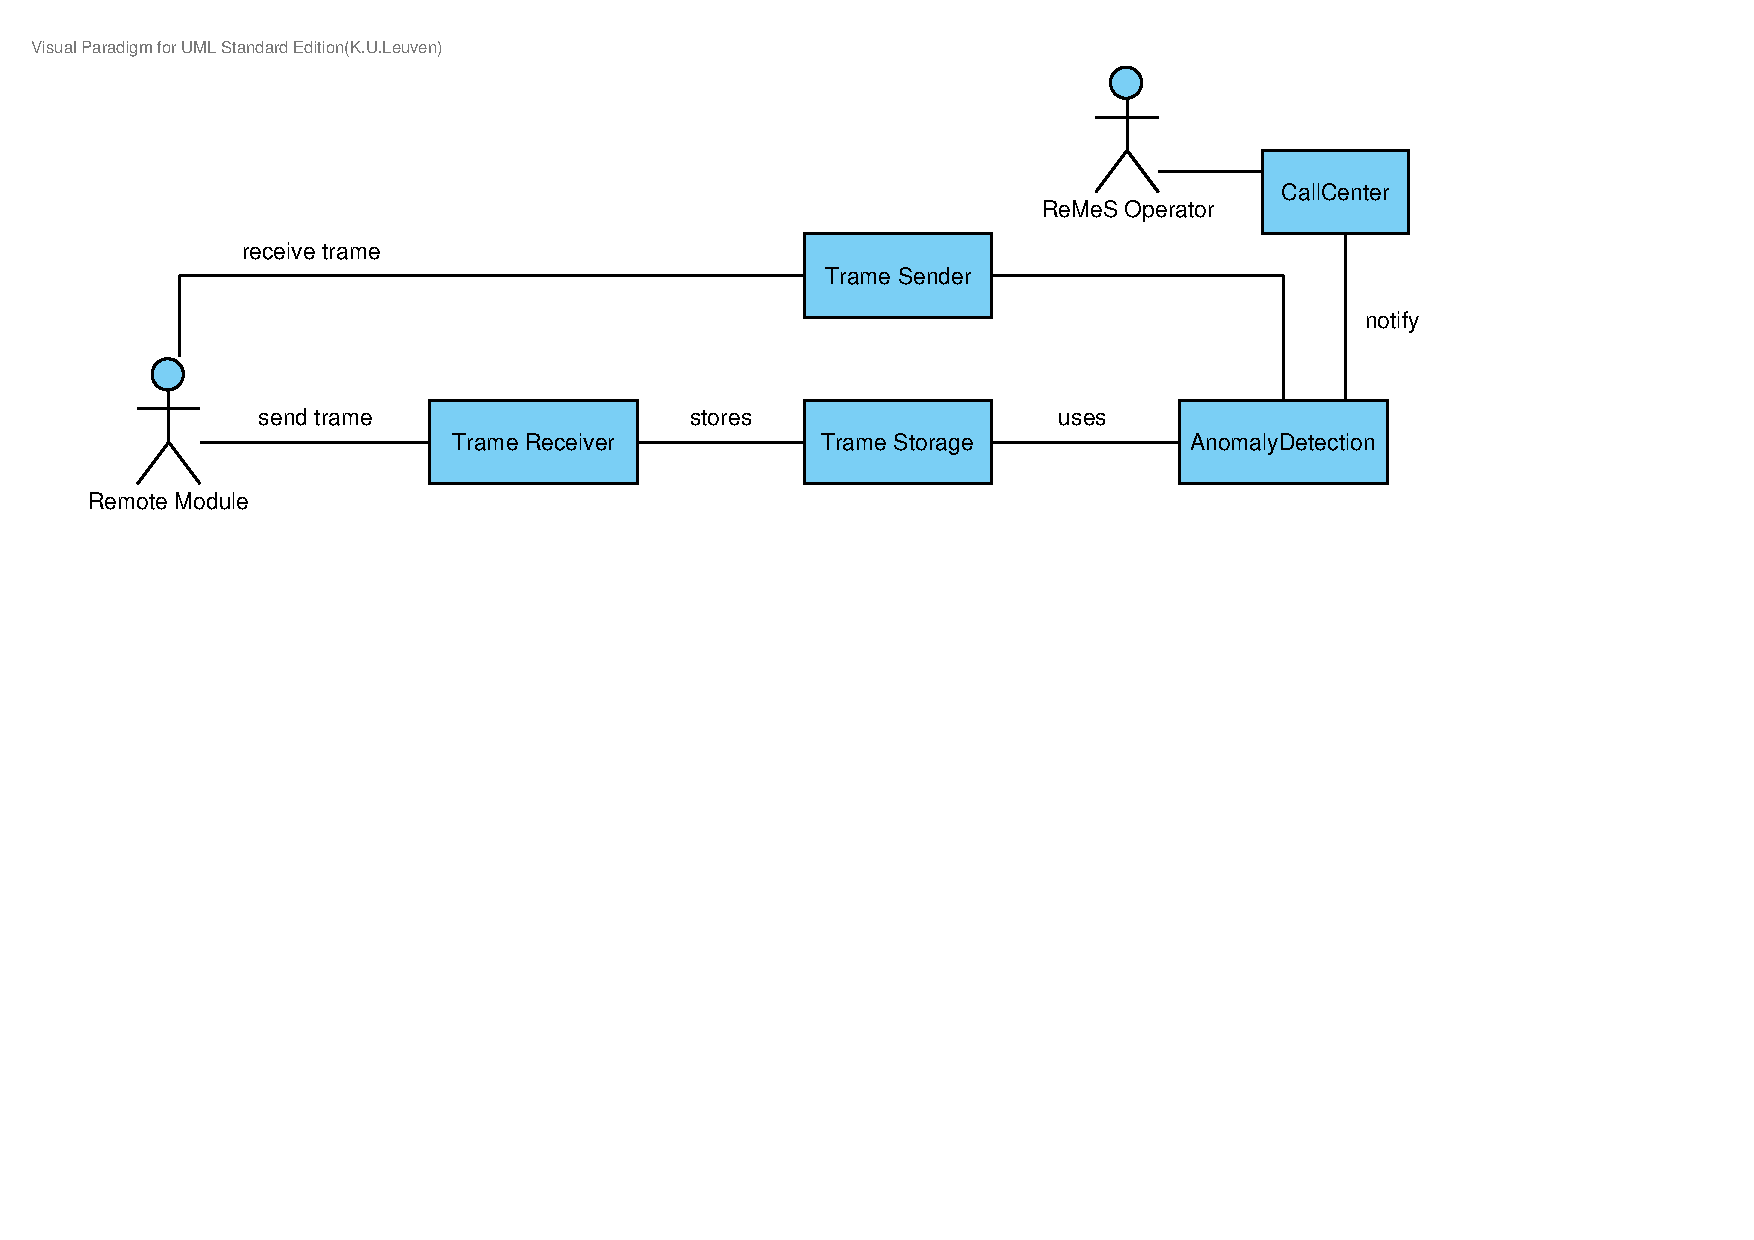
\includegraphics[width=0.6\textwidth]{figs/decomposition/whole-system/domainmodel-draft.pdf}
		\caption{Draft of the domain model used in the level 1 decomposition}
		\label{fig:dec/whole-system/draft}
	\end{centering}
\end{figure}

\subsubsection{Tactics}
\label{tactics:whole-system}

\npar After selecting the drivers for the current decomposition, one has to
choose the tactics to achieve them. Recall from section
\ref{drivers:whole-system} that the first driver was Av1. All approaches to
maintain availity involve either detection, recovery or prevention of faults.

\npar First of all to detect a fault there are three options: ping/echo,
heartbeat and exceptions. It is important to notice that the latter one is not
practical. This can be illustrated with a simple example. Suppose that a
component $c_1$ can fail while no other component $c_2$ needs a service of
$c_1$ for a duration longer than the detectioninterval of five seconds (see
Av1). For the detection we have chosen for the heartbeat tactic for
performance reasons. The ping/echo mechanism periodically requires two
messages, namely a ping and a response while the heartbeat only requires
one. Notice that only detecting a fault is insufficient, resolving the fault is
at least equally important.

\npar Once a fault has been detected, the faulting hardware must be taken out of
action and be replaced by a working version. To guarantee an uptime of 99.9\%
however, there has to a backup to take over the tasks the previously faulting
hardware was performing. As was the case in the previous paragraph, there are
many alternatives. The most frequently used ones are: active redundancy, passive
redundancy and spare. The main criterion to select one of these is the downtime
of the system. These downtimes are respectively: in the order of miliseconds,
seconds and minutes. An uptime of 99.9\% corresponds to 0.72 hours (= 43.2
minutes) of permitted downtime on a monthly basis. This number reveals potential
problems when a spare is used because there can be only less the 10 failures a
month. %TODO: argumenteren waarom active of waarom passive

\npar For performance tactics there are three categories: resource
arbitration, resource management and resource demand.

\npar If there is more than one request to gain control over a resource, there
has to be some form of scheduling. By far the most used one is a priority
scheduler where request are served earlier when they have a higher priority.
This is particulary useful for alarms to still reach the appropriate parties in
time even when the system is in overload mode. 

\npar Secondly there is resource management. To process more than one trame at a
time, concurrency can be introduced. This can be done in various ways. Several
threads can be started on one processor, on separate processors or even on
separate systems. Another possibilitiy is off course increasing the available
hardware but since this is not a very cost effective solution, this is left out
of consideration.

\npar On a lower level one could also try to minimize network overhead by
only sending small amounts of data in each trame. This is achieved by
limiting the size of the trames to 160 bytes.

\npar To conclude a small overview is given of all selected tactics for this
decomposition.

\begin{itemize}
 	\item Av1 (High): Measurement database Failure
 	\begin{itemize}
 		\item Detection: Heartbeat 
 		\item Recovery : %TODO zie eerdere todo in de tekst
 	\end{itemize}
  	\item P1 (High): Timely closure of valves
  	\begin{itemize}
  		\item Resource arbitration : Scheduling
		\item Resource management  : concurrency
		\item Resource demand      : limited tramesize
  	\end{itemize}
\end{itemize}

\subsubsection{Design Patterns}
\label{dp:whole-system}

\subsubsection{Other requirements}
\label{others:whole-system}
